\documentclass[]{article}
\usepackage{lmodern}
\usepackage{amssymb,amsmath}
\usepackage{ifxetex,ifluatex}
\usepackage{fixltx2e} % provides \textsubscript
\ifnum 0\ifxetex 1\fi\ifluatex 1\fi=0 % if pdftex
  \usepackage[T1]{fontenc}
  \usepackage[utf8]{inputenc}
\else % if luatex or xelatex
  \ifxetex
    \usepackage{mathspec}
  \else
    \usepackage{fontspec}
  \fi
  \defaultfontfeatures{Ligatures=TeX,Scale=MatchLowercase}
\fi
% use upquote if available, for straight quotes in verbatim environments
\IfFileExists{upquote.sty}{\usepackage{upquote}}{}
% use microtype if available
\IfFileExists{microtype.sty}{%
\usepackage{microtype}
\UseMicrotypeSet[protrusion]{basicmath} % disable protrusion for tt fonts
}{}
\usepackage[margin=1in]{geometry}
\usepackage{hyperref}
\hypersetup{unicode=true,
            pdftitle={Feature Importance Exploration - No IgM},
            pdfborder={0 0 0},
            breaklinks=true}
\urlstyle{same}  % don't use monospace font for urls
\usepackage{color}
\usepackage{fancyvrb}
\newcommand{\VerbBar}{|}
\newcommand{\VERB}{\Verb[commandchars=\\\{\}]}
\DefineVerbatimEnvironment{Highlighting}{Verbatim}{commandchars=\\\{\}}
% Add ',fontsize=\small' for more characters per line
\usepackage{framed}
\definecolor{shadecolor}{RGB}{248,248,248}
\newenvironment{Shaded}{\begin{snugshade}}{\end{snugshade}}
\newcommand{\KeywordTok}[1]{\textcolor[rgb]{0.13,0.29,0.53}{\textbf{#1}}}
\newcommand{\DataTypeTok}[1]{\textcolor[rgb]{0.13,0.29,0.53}{#1}}
\newcommand{\DecValTok}[1]{\textcolor[rgb]{0.00,0.00,0.81}{#1}}
\newcommand{\BaseNTok}[1]{\textcolor[rgb]{0.00,0.00,0.81}{#1}}
\newcommand{\FloatTok}[1]{\textcolor[rgb]{0.00,0.00,0.81}{#1}}
\newcommand{\ConstantTok}[1]{\textcolor[rgb]{0.00,0.00,0.00}{#1}}
\newcommand{\CharTok}[1]{\textcolor[rgb]{0.31,0.60,0.02}{#1}}
\newcommand{\SpecialCharTok}[1]{\textcolor[rgb]{0.00,0.00,0.00}{#1}}
\newcommand{\StringTok}[1]{\textcolor[rgb]{0.31,0.60,0.02}{#1}}
\newcommand{\VerbatimStringTok}[1]{\textcolor[rgb]{0.31,0.60,0.02}{#1}}
\newcommand{\SpecialStringTok}[1]{\textcolor[rgb]{0.31,0.60,0.02}{#1}}
\newcommand{\ImportTok}[1]{#1}
\newcommand{\CommentTok}[1]{\textcolor[rgb]{0.56,0.35,0.01}{\textit{#1}}}
\newcommand{\DocumentationTok}[1]{\textcolor[rgb]{0.56,0.35,0.01}{\textbf{\textit{#1}}}}
\newcommand{\AnnotationTok}[1]{\textcolor[rgb]{0.56,0.35,0.01}{\textbf{\textit{#1}}}}
\newcommand{\CommentVarTok}[1]{\textcolor[rgb]{0.56,0.35,0.01}{\textbf{\textit{#1}}}}
\newcommand{\OtherTok}[1]{\textcolor[rgb]{0.56,0.35,0.01}{#1}}
\newcommand{\FunctionTok}[1]{\textcolor[rgb]{0.00,0.00,0.00}{#1}}
\newcommand{\VariableTok}[1]{\textcolor[rgb]{0.00,0.00,0.00}{#1}}
\newcommand{\ControlFlowTok}[1]{\textcolor[rgb]{0.13,0.29,0.53}{\textbf{#1}}}
\newcommand{\OperatorTok}[1]{\textcolor[rgb]{0.81,0.36,0.00}{\textbf{#1}}}
\newcommand{\BuiltInTok}[1]{#1}
\newcommand{\ExtensionTok}[1]{#1}
\newcommand{\PreprocessorTok}[1]{\textcolor[rgb]{0.56,0.35,0.01}{\textit{#1}}}
\newcommand{\AttributeTok}[1]{\textcolor[rgb]{0.77,0.63,0.00}{#1}}
\newcommand{\RegionMarkerTok}[1]{#1}
\newcommand{\InformationTok}[1]{\textcolor[rgb]{0.56,0.35,0.01}{\textbf{\textit{#1}}}}
\newcommand{\WarningTok}[1]{\textcolor[rgb]{0.56,0.35,0.01}{\textbf{\textit{#1}}}}
\newcommand{\AlertTok}[1]{\textcolor[rgb]{0.94,0.16,0.16}{#1}}
\newcommand{\ErrorTok}[1]{\textcolor[rgb]{0.64,0.00,0.00}{\textbf{#1}}}
\newcommand{\NormalTok}[1]{#1}
\usepackage{graphicx,grffile}
\makeatletter
\def\maxwidth{\ifdim\Gin@nat@width>\linewidth\linewidth\else\Gin@nat@width\fi}
\def\maxheight{\ifdim\Gin@nat@height>\textheight\textheight\else\Gin@nat@height\fi}
\makeatother
% Scale images if necessary, so that they will not overflow the page
% margins by default, and it is still possible to overwrite the defaults
% using explicit options in \includegraphics[width, height, ...]{}
\setkeys{Gin}{width=\maxwidth,height=\maxheight,keepaspectratio}
\IfFileExists{parskip.sty}{%
\usepackage{parskip}
}{% else
\setlength{\parindent}{0pt}
\setlength{\parskip}{6pt plus 2pt minus 1pt}
}
\setlength{\emergencystretch}{3em}  % prevent overfull lines
\providecommand{\tightlist}{%
  \setlength{\itemsep}{0pt}\setlength{\parskip}{0pt}}
\setcounter{secnumdepth}{0}
% Redefines (sub)paragraphs to behave more like sections
\ifx\paragraph\undefined\else
\let\oldparagraph\paragraph
\renewcommand{\paragraph}[1]{\oldparagraph{#1}\mbox{}}
\fi
\ifx\subparagraph\undefined\else
\let\oldsubparagraph\subparagraph
\renewcommand{\subparagraph}[1]{\oldsubparagraph{#1}\mbox{}}
\fi

%%% Use protect on footnotes to avoid problems with footnotes in titles
\let\rmarkdownfootnote\footnote%
\def\footnote{\protect\rmarkdownfootnote}

%%% Change title format to be more compact
\usepackage{titling}

% Create subtitle command for use in maketitle
\providecommand{\subtitle}[1]{
  \posttitle{
    \begin{center}\large#1\end{center}
    }
}

\setlength{\droptitle}{-2em}

  \title{Feature Importance Exploration - No IgM}
    \pretitle{\vspace{\droptitle}\centering\huge}
  \posttitle{\par}
    \author{}
    \preauthor{}\postauthor{}
    \date{}
    \predate{}\postdate{}
  

\begin{document}
\maketitle

\section{Import libraries}\label{import-libraries}

\section{Load Data}\label{load-data}

This block performs the following operations:

\begin{enumerate}
\def\labelenumi{\arabic{enumi}.}
\tightlist
\item
  Loads the raw data.
\item
  Selects the desired predictor variables.
\item
  Drops rows with missing data.
\item
  Prepares the target variable, transforming it from 4 classes to 2.
\end{enumerate}

\begin{Shaded}
\begin{Highlighting}[]
\KeywordTok{set.seed}\NormalTok{(}\DecValTok{88}\NormalTok{)}
\NormalTok{data_csv <-}\StringTok{ }\KeywordTok{here}\NormalTok{(}\StringTok{"data"}\NormalTok{, }\StringTok{"raw"}\NormalTok{, }\StringTok{"final_data.csv"}\NormalTok{)}
\NormalTok{df <-}\StringTok{ }\KeywordTok{read.csv}\NormalTok{(data_csv)}

\NormalTok{df <-}\StringTok{ }\NormalTok{df }\OperatorTok\StringTok{ }
\StringTok{  }\KeywordTok{select}\NormalTok{(}\OperatorTok{-}\NormalTok{Sample) }\OperatorTok\StringTok{ }
\StringTok{  }\KeywordTok{drop_na}\NormalTok{() }\OperatorTok\StringTok{ }
\StringTok{  }\KeywordTok{mutate}\NormalTok{(}\DataTypeTok{Cohort =} \KeywordTok{factor}\NormalTok{(}\KeywordTok{if_else}\NormalTok{(Cohort }\OperatorTok\StringTok{ }\KeywordTok{c}\NormalTok{(}\StringTok{"PP"}\NormalTok{, }\StringTok{"NP"}\NormalTok{), }\StringTok{"Primary"}\NormalTok{, }\StringTok{"Latent"}\NormalTok{)))}
\end{Highlighting}
\end{Shaded}

\section{Preprocessing}\label{preprocessing}

The following block uses the \texttt{recipes} library to log scale and
normalize the predictors between 0 and 1.

\begin{Shaded}
\begin{Highlighting}[]
\NormalTok{rec_obj <-}\StringTok{ }\KeywordTok{recipe}\NormalTok{(Cohort }\OperatorTok{~}\StringTok{ }\NormalTok{., }\DataTypeTok{data =}\NormalTok{ df)}

\NormalTok{normalizer <-}\StringTok{ }\NormalTok{rec_obj }\OperatorTok\StringTok{ }
\StringTok{  }\KeywordTok{step_log}\NormalTok{(}\KeywordTok{all_predictors}\NormalTok{()) }\OperatorTok\StringTok{ }
\StringTok{  }\KeywordTok{step_range}\NormalTok{(}\KeywordTok{all_predictors}\NormalTok{(), }\DataTypeTok{min =} \DecValTok{0}\NormalTok{, }\DataTypeTok{max =} \DecValTok{1}\NormalTok{)}

\NormalTok{trained_rec <-}\StringTok{ }\KeywordTok{prep}\NormalTok{(normalizer, }\DataTypeTok{training =}\NormalTok{ df)}

\NormalTok{norm_df <-}\StringTok{ }\KeywordTok{bake}\NormalTok{(trained_rec, df)}
\end{Highlighting}
\end{Shaded}

\section{Predicting}\label{predicting}

The following block performs 10-fold cross validation using lasso
regression with the \texttt{glmnet} package. \texttt{mod\_df} removes
all \texttt{IgM} features.

\begin{Shaded}
\begin{Highlighting}[]
\CommentTok{# mod_df <- norm_df}
\NormalTok{mod_df <-}\StringTok{ }\NormalTok{norm_df[, }\OperatorTok{-}\KeywordTok{grep}\NormalTok{(}\StringTok{"^IgM"}\NormalTok{, }\KeywordTok{colnames}\NormalTok{(norm_df))]}

\NormalTok{perm_df <-}\StringTok{ }\NormalTok{mod_df }\OperatorTok\StringTok{ }
\StringTok{  }\KeywordTok{mutate}\NormalTok{(}\DataTypeTok{permCohort =} \KeywordTok{sample}\NormalTok{(mod_df}\OperatorTok{$}\NormalTok{Cohort), }\KeywordTok{nrow}\NormalTok{(mod_df)) }\OperatorTok\StringTok{ }
\StringTok{  }\KeywordTok{select}\NormalTok{(}\OperatorTok{-}\NormalTok{Cohort)}
\end{Highlighting}
\end{Shaded}

\begin{Shaded}
\begin{Highlighting}[]
\NormalTok{myGrid =}\StringTok{ }\KeywordTok{expand.grid}\NormalTok{(}
  \DataTypeTok{alpha =} \DecValTok{1}\NormalTok{,}
  \DataTypeTok{lambda =} \KeywordTok{seq}\NormalTok{(}\FloatTok{0.0001}\NormalTok{, }\DecValTok{1}\NormalTok{, }\DataTypeTok{length =} \DecValTok{100}\NormalTok{)}
\NormalTok{)}

\NormalTok{model <-}\StringTok{ }\KeywordTok{train}\NormalTok{(}
\NormalTok{  Cohort }\OperatorTok{~}\StringTok{ }\NormalTok{., }
\NormalTok{  mod_df, }
  \DataTypeTok{method =} \StringTok{'glmnet'}\NormalTok{,}
  \DataTypeTok{tuneGrid =}\NormalTok{ myGrid,}
  \DataTypeTok{trControl =} \KeywordTok{trainControl}\NormalTok{(}
    \DataTypeTok{method =} \StringTok{"cv"}\NormalTok{,}
    \DataTypeTok{number =} \DecValTok{10}\NormalTok{,}
    \DataTypeTok{summaryFunction =}\NormalTok{ twoClassSummary,}
    \DataTypeTok{classProbs =} \OtherTok{TRUE}\NormalTok{,}
    \DataTypeTok{verboseIter =} \OtherTok{TRUE}
\NormalTok{  )}
\NormalTok{)}
\end{Highlighting}
\end{Shaded}

\begin{verbatim}
## Warning in train.default(x, y, weights = w, ...): The metric "Accuracy" was
## not in the result set. ROC will be used instead.
\end{verbatim}

\begin{verbatim}
## + Fold01: alpha=1, lambda=1 
## - Fold01: alpha=1, lambda=1 
## + Fold02: alpha=1, lambda=1 
## - Fold02: alpha=1, lambda=1 
## + Fold03: alpha=1, lambda=1 
## - Fold03: alpha=1, lambda=1 
## + Fold04: alpha=1, lambda=1 
## - Fold04: alpha=1, lambda=1 
## + Fold05: alpha=1, lambda=1 
## - Fold05: alpha=1, lambda=1 
## + Fold06: alpha=1, lambda=1 
## - Fold06: alpha=1, lambda=1 
## + Fold07: alpha=1, lambda=1 
## - Fold07: alpha=1, lambda=1 
## + Fold08: alpha=1, lambda=1 
## - Fold08: alpha=1, lambda=1 
## + Fold09: alpha=1, lambda=1 
## - Fold09: alpha=1, lambda=1 
## + Fold10: alpha=1, lambda=1 
## - Fold10: alpha=1, lambda=1 
## Aggregating results
## Selecting tuning parameters
## Fitting alpha = 1, lambda = 0.101 on full training set
\end{verbatim}

\begin{Shaded}
\begin{Highlighting}[]
\NormalTok{model}
\end{Highlighting}
\end{Shaded}

\begin{verbatim}
## glmnet 
## 
## 101 samples
## 214 predictors
##   2 classes: 'Latent', 'Primary' 
## 
## No pre-processing
## Resampling: Cross-Validated (10 fold) 
## Summary of sample sizes: 90, 91, 92, 91, 91, 91, ... 
## Resampling results across tuning parameters:
## 
##   lambda  ROC        Sens       Spec 
##   0.0001  0.9626667  0.9300000  0.880
##   0.0102  0.9626667  0.9300000  0.880
##   0.0203  0.9626667  0.9466667  0.860
##   0.0304  0.9746667  0.9466667  0.860
##   0.0405  0.9786667  0.9466667  0.880
##   0.0506  0.9786667  0.9666667  0.880
##   0.0607  0.9826667  0.9666667  0.880
##   0.0708  0.9793333  0.9666667  0.855
##   0.0809  0.9833333  0.9500000  0.835
##   0.0910  0.9833333  0.9500000  0.835
##   0.1011  0.9833333  0.9500000  0.815
##   0.1112  0.9783333  0.9500000  0.815
##   0.1213  0.9783333  0.9500000  0.815
##   0.1314  0.9783333  0.9333333  0.815
##   0.1415  0.9743333  0.9333333  0.815
##   0.1516  0.9743333  0.9333333  0.815
##   0.1617  0.9743333  0.9333333  0.815
##   0.1718  0.9743333  0.9333333  0.795
##   0.1819  0.9743333  0.9333333  0.795
##   0.1920  0.9710000  0.9333333  0.795
##   0.2021  0.9743333  0.9333333  0.795
##   0.2122  0.9743333  0.9333333  0.795
##   0.2223  0.9743333  0.9333333  0.795
##   0.2324  0.9743333  0.9333333  0.795
##   0.2425  0.9670000  0.9333333  0.775
##   0.2526  0.9676667  0.9333333  0.755
##   0.2627  0.9693333  0.9333333  0.715
##   0.2728  0.9653333  0.9333333  0.715
##   0.2829  0.9613333  0.9333333  0.675
##   0.2930  0.9498333  0.9333333  0.610
##   0.3031  0.9498333  0.9333333  0.525
##   0.3132  0.9385000  0.9333333  0.440
##   0.3233  0.9385000  0.9333333  0.395
##   0.3334  0.9345000  0.9500000  0.220
##   0.3435  0.9378333  1.0000000  0.045
##   0.3536  0.7878333  1.0000000  0.000
##   0.3637  0.5820000  1.0000000  0.000
##   0.3738  0.5000000  1.0000000  0.000
##   0.3839  0.5000000  1.0000000  0.000
##   0.3940  0.5000000  1.0000000  0.000
##   0.4041  0.5000000  1.0000000  0.000
##   0.4142  0.5000000  1.0000000  0.000
##   0.4243  0.5000000  1.0000000  0.000
##   0.4344  0.5000000  1.0000000  0.000
##   0.4445  0.5000000  1.0000000  0.000
##   0.4546  0.5000000  1.0000000  0.000
##   0.4647  0.5000000  1.0000000  0.000
##   0.4748  0.5000000  1.0000000  0.000
##   0.4849  0.5000000  1.0000000  0.000
##   0.4950  0.5000000  1.0000000  0.000
##   0.5051  0.5000000  1.0000000  0.000
##   0.5152  0.5000000  1.0000000  0.000
##   0.5253  0.5000000  1.0000000  0.000
##   0.5354  0.5000000  1.0000000  0.000
##   0.5455  0.5000000  1.0000000  0.000
##   0.5556  0.5000000  1.0000000  0.000
##   0.5657  0.5000000  1.0000000  0.000
##   0.5758  0.5000000  1.0000000  0.000
##   0.5859  0.5000000  1.0000000  0.000
##   0.5960  0.5000000  1.0000000  0.000
##   0.6061  0.5000000  1.0000000  0.000
##   0.6162  0.5000000  1.0000000  0.000
##   0.6263  0.5000000  1.0000000  0.000
##   0.6364  0.5000000  1.0000000  0.000
##   0.6465  0.5000000  1.0000000  0.000
##   0.6566  0.5000000  1.0000000  0.000
##   0.6667  0.5000000  1.0000000  0.000
##   0.6768  0.5000000  1.0000000  0.000
##   0.6869  0.5000000  1.0000000  0.000
##   0.6970  0.5000000  1.0000000  0.000
##   0.7071  0.5000000  1.0000000  0.000
##   0.7172  0.5000000  1.0000000  0.000
##   0.7273  0.5000000  1.0000000  0.000
##   0.7374  0.5000000  1.0000000  0.000
##   0.7475  0.5000000  1.0000000  0.000
##   0.7576  0.5000000  1.0000000  0.000
##   0.7677  0.5000000  1.0000000  0.000
##   0.7778  0.5000000  1.0000000  0.000
##   0.7879  0.5000000  1.0000000  0.000
##   0.7980  0.5000000  1.0000000  0.000
##   0.8081  0.5000000  1.0000000  0.000
##   0.8182  0.5000000  1.0000000  0.000
##   0.8283  0.5000000  1.0000000  0.000
##   0.8384  0.5000000  1.0000000  0.000
##   0.8485  0.5000000  1.0000000  0.000
##   0.8586  0.5000000  1.0000000  0.000
##   0.8687  0.5000000  1.0000000  0.000
##   0.8788  0.5000000  1.0000000  0.000
##   0.8889  0.5000000  1.0000000  0.000
##   0.8990  0.5000000  1.0000000  0.000
##   0.9091  0.5000000  1.0000000  0.000
##   0.9192  0.5000000  1.0000000  0.000
##   0.9293  0.5000000  1.0000000  0.000
##   0.9394  0.5000000  1.0000000  0.000
##   0.9495  0.5000000  1.0000000  0.000
##   0.9596  0.5000000  1.0000000  0.000
##   0.9697  0.5000000  1.0000000  0.000
##   0.9798  0.5000000  1.0000000  0.000
##   0.9899  0.5000000  1.0000000  0.000
##   1.0000  0.5000000  1.0000000  0.000
## 
## Tuning parameter 'alpha' was held constant at a value of 1
## ROC was used to select the optimal model using the largest value.
## The final values used for the model were alpha = 1 and lambda = 0.1011.
\end{verbatim}

The following block repeats the operation in the previous block with
permuted labels in order to simulate the null hypothesis.

\begin{Shaded}
\begin{Highlighting}[]
\NormalTok{permModel <-}\StringTok{ }\KeywordTok{train}\NormalTok{(}
\NormalTok{  permCohort }\OperatorTok{~}\StringTok{ }\NormalTok{., }
\NormalTok{  perm_df, }
  \DataTypeTok{method =} \StringTok{'glmnet'}\NormalTok{,}
  \DataTypeTok{tuneGrid =}\NormalTok{ myGrid,}
  \DataTypeTok{trControl =} \KeywordTok{trainControl}\NormalTok{(}
    \DataTypeTok{method =} \StringTok{"cv"}\NormalTok{,}
    \DataTypeTok{number =} \DecValTok{10}\NormalTok{,}
    \DataTypeTok{summaryFunction =}\NormalTok{ twoClassSummary,}
    \DataTypeTok{classProbs =} \OtherTok{TRUE}\NormalTok{,}
    \DataTypeTok{verboseIter =} \OtherTok{TRUE}
\NormalTok{  )}
\NormalTok{)}
\end{Highlighting}
\end{Shaded}

\begin{verbatim}
## Warning in train.default(x, y, weights = w, ...): The metric "Accuracy" was
## not in the result set. ROC will be used instead.
\end{verbatim}

\begin{verbatim}
## + Fold01: alpha=1, lambda=1 
## - Fold01: alpha=1, lambda=1 
## + Fold02: alpha=1, lambda=1 
## - Fold02: alpha=1, lambda=1 
## + Fold03: alpha=1, lambda=1 
## - Fold03: alpha=1, lambda=1 
## + Fold04: alpha=1, lambda=1 
## - Fold04: alpha=1, lambda=1 
## + Fold05: alpha=1, lambda=1 
## - Fold05: alpha=1, lambda=1 
## + Fold06: alpha=1, lambda=1 
## - Fold06: alpha=1, lambda=1 
## + Fold07: alpha=1, lambda=1 
## - Fold07: alpha=1, lambda=1 
## + Fold08: alpha=1, lambda=1 
## - Fold08: alpha=1, lambda=1 
## + Fold09: alpha=1, lambda=1 
## - Fold09: alpha=1, lambda=1 
## + Fold10: alpha=1, lambda=1 
## - Fold10: alpha=1, lambda=1 
## Aggregating results
## Selecting tuning parameters
## Fitting alpha = 1, lambda = 0.091 on full training set
\end{verbatim}

\begin{Shaded}
\begin{Highlighting}[]
\NormalTok{permModel}
\end{Highlighting}
\end{Shaded}

\begin{verbatim}
## glmnet 
## 
## 101 samples
## 215 predictors
##   2 classes: 'Latent', 'Primary' 
## 
## No pre-processing
## Resampling: Cross-Validated (10 fold) 
## Summary of sample sizes: 91, 91, 90, 91, 91, 90, ... 
## Resampling results across tuning parameters:
## 
##   lambda  ROC        Sens       Spec 
##   0.0001  0.5341667  0.6066667  0.455
##   0.0102  0.5211667  0.5900000  0.455
##   0.0203  0.5386667  0.5800000  0.495
##   0.0304  0.5536667  0.5600000  0.465
##   0.0405  0.5268333  0.5800000  0.445
##   0.0506  0.5038333  0.5966667  0.400
##   0.0607  0.5168333  0.6500000  0.320
##   0.0708  0.5381667  0.6700000  0.320
##   0.0809  0.5535000  0.7100000  0.300
##   0.0910  0.5573333  0.8000000  0.250
##   0.1011  0.5243333  0.8766667  0.250
##   0.1112  0.5258333  0.8766667  0.090
##   0.1213  0.5200000  0.9333333  0.045
##   0.1314  0.5078333  0.9500000  0.000
##   0.1415  0.4598333  0.9666667  0.000
##   0.1516  0.4766667  0.9833333  0.000
##   0.1617  0.4766667  0.9833333  0.000
##   0.1718  0.4766667  0.9833333  0.000
##   0.1819  0.4766667  1.0000000  0.000
##   0.1920  0.5000000  1.0000000  0.000
##   0.2021  0.5000000  1.0000000  0.000
##   0.2122  0.5000000  1.0000000  0.000
##   0.2223  0.5000000  1.0000000  0.000
##   0.2324  0.5000000  1.0000000  0.000
##   0.2425  0.5000000  1.0000000  0.000
##   0.2526  0.5000000  1.0000000  0.000
##   0.2627  0.5000000  1.0000000  0.000
##   0.2728  0.5000000  1.0000000  0.000
##   0.2829  0.5000000  1.0000000  0.000
##   0.2930  0.5000000  1.0000000  0.000
##   0.3031  0.5000000  1.0000000  0.000
##   0.3132  0.5000000  1.0000000  0.000
##   0.3233  0.5000000  1.0000000  0.000
##   0.3334  0.5000000  1.0000000  0.000
##   0.3435  0.5000000  1.0000000  0.000
##   0.3536  0.5000000  1.0000000  0.000
##   0.3637  0.5000000  1.0000000  0.000
##   0.3738  0.5000000  1.0000000  0.000
##   0.3839  0.5000000  1.0000000  0.000
##   0.3940  0.5000000  1.0000000  0.000
##   0.4041  0.5000000  1.0000000  0.000
##   0.4142  0.5000000  1.0000000  0.000
##   0.4243  0.5000000  1.0000000  0.000
##   0.4344  0.5000000  1.0000000  0.000
##   0.4445  0.5000000  1.0000000  0.000
##   0.4546  0.5000000  1.0000000  0.000
##   0.4647  0.5000000  1.0000000  0.000
##   0.4748  0.5000000  1.0000000  0.000
##   0.4849  0.5000000  1.0000000  0.000
##   0.4950  0.5000000  1.0000000  0.000
##   0.5051  0.5000000  1.0000000  0.000
##   0.5152  0.5000000  1.0000000  0.000
##   0.5253  0.5000000  1.0000000  0.000
##   0.5354  0.5000000  1.0000000  0.000
##   0.5455  0.5000000  1.0000000  0.000
##   0.5556  0.5000000  1.0000000  0.000
##   0.5657  0.5000000  1.0000000  0.000
##   0.5758  0.5000000  1.0000000  0.000
##   0.5859  0.5000000  1.0000000  0.000
##   0.5960  0.5000000  1.0000000  0.000
##   0.6061  0.5000000  1.0000000  0.000
##   0.6162  0.5000000  1.0000000  0.000
##   0.6263  0.5000000  1.0000000  0.000
##   0.6364  0.5000000  1.0000000  0.000
##   0.6465  0.5000000  1.0000000  0.000
##   0.6566  0.5000000  1.0000000  0.000
##   0.6667  0.5000000  1.0000000  0.000
##   0.6768  0.5000000  1.0000000  0.000
##   0.6869  0.5000000  1.0000000  0.000
##   0.6970  0.5000000  1.0000000  0.000
##   0.7071  0.5000000  1.0000000  0.000
##   0.7172  0.5000000  1.0000000  0.000
##   0.7273  0.5000000  1.0000000  0.000
##   0.7374  0.5000000  1.0000000  0.000
##   0.7475  0.5000000  1.0000000  0.000
##   0.7576  0.5000000  1.0000000  0.000
##   0.7677  0.5000000  1.0000000  0.000
##   0.7778  0.5000000  1.0000000  0.000
##   0.7879  0.5000000  1.0000000  0.000
##   0.7980  0.5000000  1.0000000  0.000
##   0.8081  0.5000000  1.0000000  0.000
##   0.8182  0.5000000  1.0000000  0.000
##   0.8283  0.5000000  1.0000000  0.000
##   0.8384  0.5000000  1.0000000  0.000
##   0.8485  0.5000000  1.0000000  0.000
##   0.8586  0.5000000  1.0000000  0.000
##   0.8687  0.5000000  1.0000000  0.000
##   0.8788  0.5000000  1.0000000  0.000
##   0.8889  0.5000000  1.0000000  0.000
##   0.8990  0.5000000  1.0000000  0.000
##   0.9091  0.5000000  1.0000000  0.000
##   0.9192  0.5000000  1.0000000  0.000
##   0.9293  0.5000000  1.0000000  0.000
##   0.9394  0.5000000  1.0000000  0.000
##   0.9495  0.5000000  1.0000000  0.000
##   0.9596  0.5000000  1.0000000  0.000
##   0.9697  0.5000000  1.0000000  0.000
##   0.9798  0.5000000  1.0000000  0.000
##   0.9899  0.5000000  1.0000000  0.000
##   1.0000  0.5000000  1.0000000  0.000
## 
## Tuning parameter 'alpha' was held constant at a value of 1
## ROC was used to select the optimal model using the largest value.
## The final values used for the model were alpha = 1 and lambda = 0.091.
\end{verbatim}

The following block plots the ROC-AUC metric distributions for the real
and permuted versions of the \texttt{glmnet} model as violin plots.

\begin{Shaded}
\begin{Highlighting}[]
\NormalTok{realSamps <-}\StringTok{ }\NormalTok{model}\OperatorTok{$}\NormalTok{resample }\OperatorTok\StringTok{ }
\StringTok{  }\KeywordTok{mutate}\NormalTok{(}\DataTypeTok{model =} \StringTok{"Real"}\NormalTok{)}

\NormalTok{permSamps <-}\StringTok{ }\NormalTok{permModel}\OperatorTok{$}\NormalTok{resample }\OperatorTok\StringTok{ }
\StringTok{  }\KeywordTok{mutate}\NormalTok{(}\DataTypeTok{model =} \StringTok{"Permuted"}\NormalTok{)}

\NormalTok{box_df <-}\StringTok{ }\KeywordTok{bind_rows}\NormalTok{(realSamps, permSamps)}

\KeywordTok{ggplot}\NormalTok{(box_df, }\KeywordTok{aes}\NormalTok{(}\KeywordTok{fct_relevel}\NormalTok{(model, }\KeywordTok{c}\NormalTok{(}\StringTok{"Real"}\NormalTok{, }\StringTok{"Permuted"}\NormalTok{)), ROC)) }\OperatorTok{+}
\StringTok{  }\KeywordTok{geom_violin}\NormalTok{() }\OperatorTok{+}
\StringTok{  }\KeywordTok{expand_limits}\NormalTok{(}\DataTypeTok{y =} \DecValTok{0}\NormalTok{) }\OperatorTok{+}
\StringTok{  }\KeywordTok{labs}\NormalTok{(}\DataTypeTok{title =} \StringTok{"ROC Distribution by CV Fold"}\NormalTok{,}
       \DataTypeTok{x =} \StringTok{"Model Run"}\NormalTok{,}
       \DataTypeTok{y =} \StringTok{"ROC AUC"}\NormalTok{)}
\end{Highlighting}
\end{Shaded}

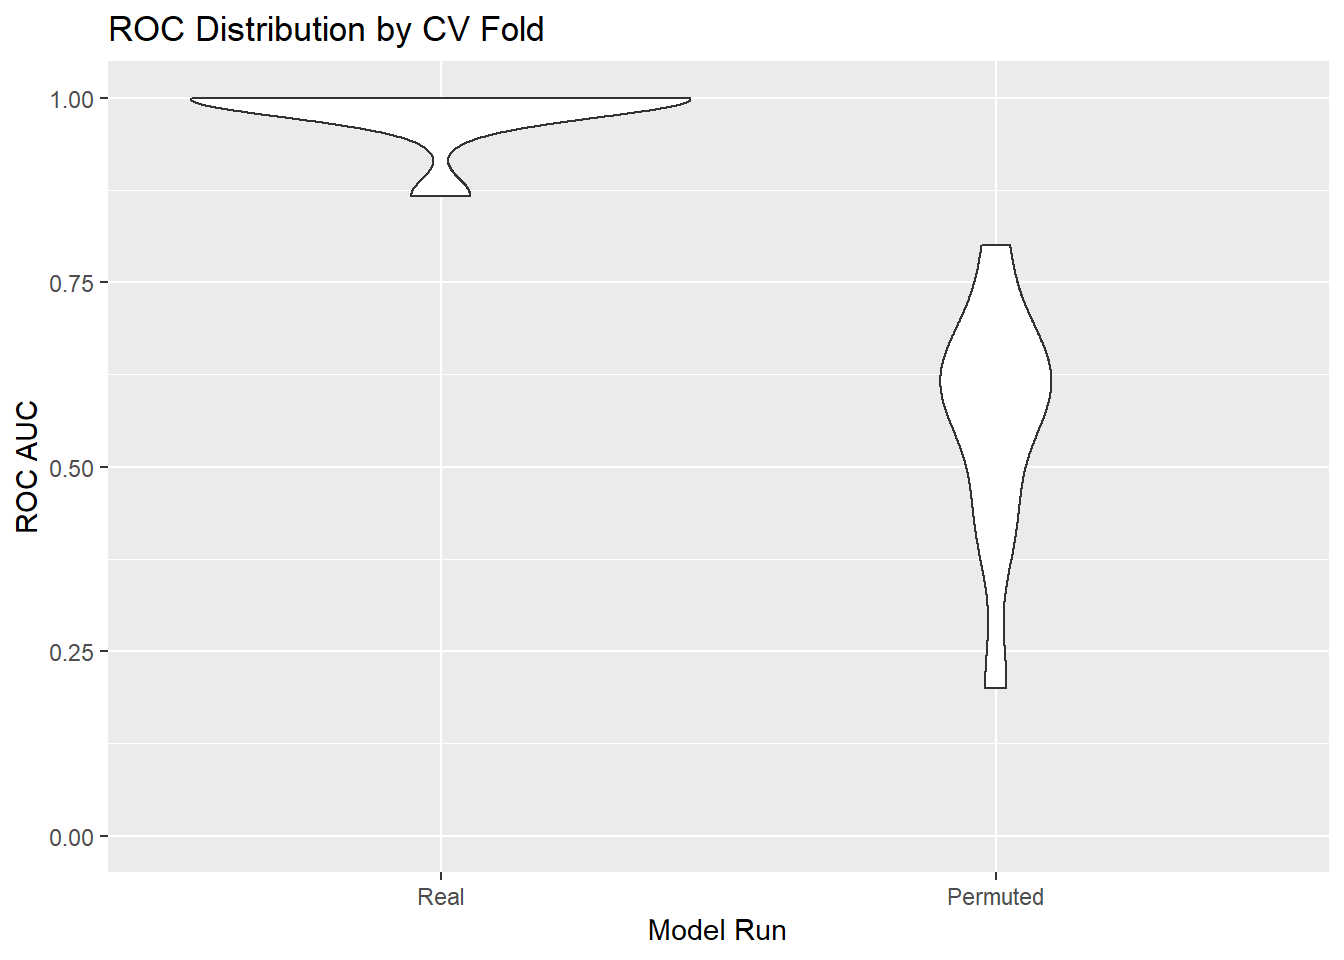
\includegraphics{report_files/figure-latex/unnamed-chunk-7-1.pdf}

The following block plots the coefficients from the best model
identified by \texttt{glmnet}.

\begin{Shaded}
\begin{Highlighting}[]
\CommentTok{# Predictor}
\NormalTok{feature_matrix <-}\StringTok{ }\NormalTok{mod_df }\OperatorTok\StringTok{ }
\StringTok{  }\KeywordTok{select}\NormalTok{(}\OperatorTok{-}\NormalTok{Cohort) }\OperatorTok\StringTok{ }
\StringTok{  }\KeywordTok{as.matrix}\NormalTok{()}

\CommentTok{# Target}
\NormalTok{cohort <-}\StringTok{ }\NormalTok{mod_df}\OperatorTok{$}\NormalTok{Cohort}

\NormalTok{lasso_fit <-}\StringTok{ }\KeywordTok{glmnet}\NormalTok{(feature_matrix, cohort, }\DataTypeTok{family =} \StringTok{"binomial"}\NormalTok{, }\DataTypeTok{alpha =} \DecValTok{1}\NormalTok{, }\DataTypeTok{lambda =}\NormalTok{ model}\OperatorTok{$}\NormalTok{bestTune}\OperatorTok{$}\NormalTok{lambda)}

\NormalTok{lasso_fit }\OperatorTok\StringTok{ }
\StringTok{  }\KeywordTok{tidy}\NormalTok{() }\OperatorTok\StringTok{ }
\StringTok{  }\KeywordTok{arrange}\NormalTok{(}\KeywordTok{desc}\NormalTok{(estimate)) }\OperatorTok\StringTok{ }
\StringTok{  }\KeywordTok{filter}\NormalTok{(term }\OperatorTok{!=}\StringTok{ "(Intercept)"}\NormalTok{) }\OperatorTok\StringTok{ }
\StringTok{  }\KeywordTok{mutate}\NormalTok{(}\DataTypeTok{term =} \KeywordTok{fct_reorder}\NormalTok{(term, estimate)) }\OperatorTok\StringTok{ }
\StringTok{  }\KeywordTok{ggplot}\NormalTok{(}\KeywordTok{aes}\NormalTok{(term, estimate)) }\OperatorTok{+}
\StringTok{  }\KeywordTok{geom_col}\NormalTok{() }\OperatorTok{+}
\StringTok{  }\KeywordTok{coord_flip}\NormalTok{() }\OperatorTok{+}
\StringTok{  }\KeywordTok{labs}\NormalTok{(}\DataTypeTok{title =} \StringTok{"Coefficients in predictive model"}\NormalTok{,}
       \DataTypeTok{subtitle =} \StringTok{"Based on LASSO regression"}\NormalTok{,}
       \DataTypeTok{x =} \StringTok{""}\NormalTok{,}
       \DataTypeTok{y =} \StringTok{"Coefficient"}\NormalTok{)}
\end{Highlighting}
\end{Shaded}

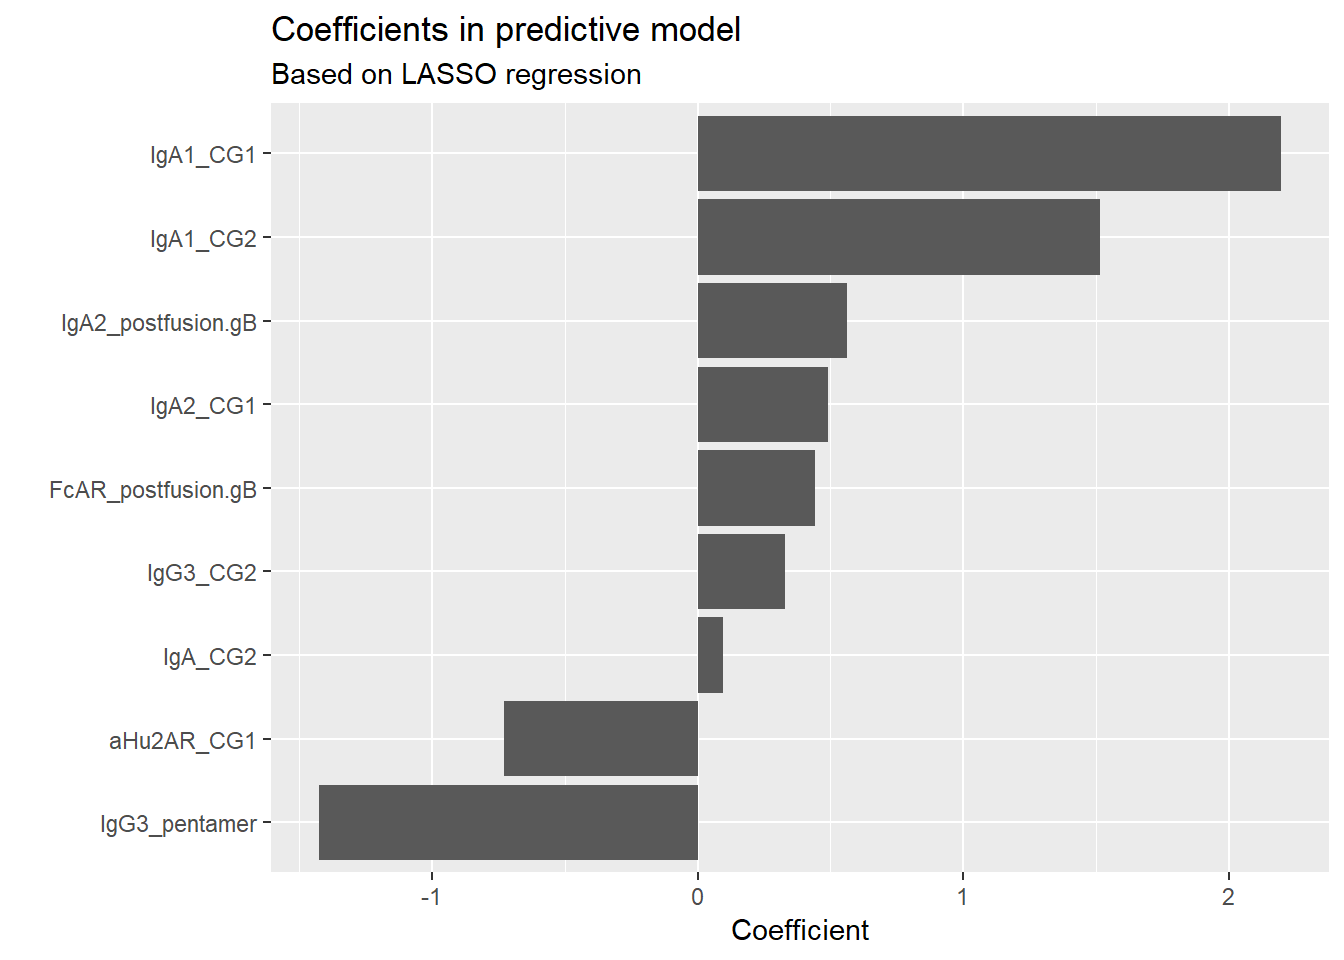
\includegraphics{report_files/figure-latex/unnamed-chunk-8-1.pdf}

\section{Evaluating}\label{evaluating}

This block evaluates the performance of the model using the ROC metric.

\begin{Shaded}
\begin{Highlighting}[]
\KeywordTok{library}\NormalTok{(caTools)}
\NormalTok{preds <-}\StringTok{ }\KeywordTok{predict}\NormalTok{(lasso_fit, feature_matrix, }\DataTypeTok{type =} \StringTok{"response"}\NormalTok{)}

\KeywordTok{colAUC}\NormalTok{(preds, cohort, }\DataTypeTok{plotROC =} \OtherTok{TRUE}\NormalTok{)}
\end{Highlighting}
\end{Shaded}

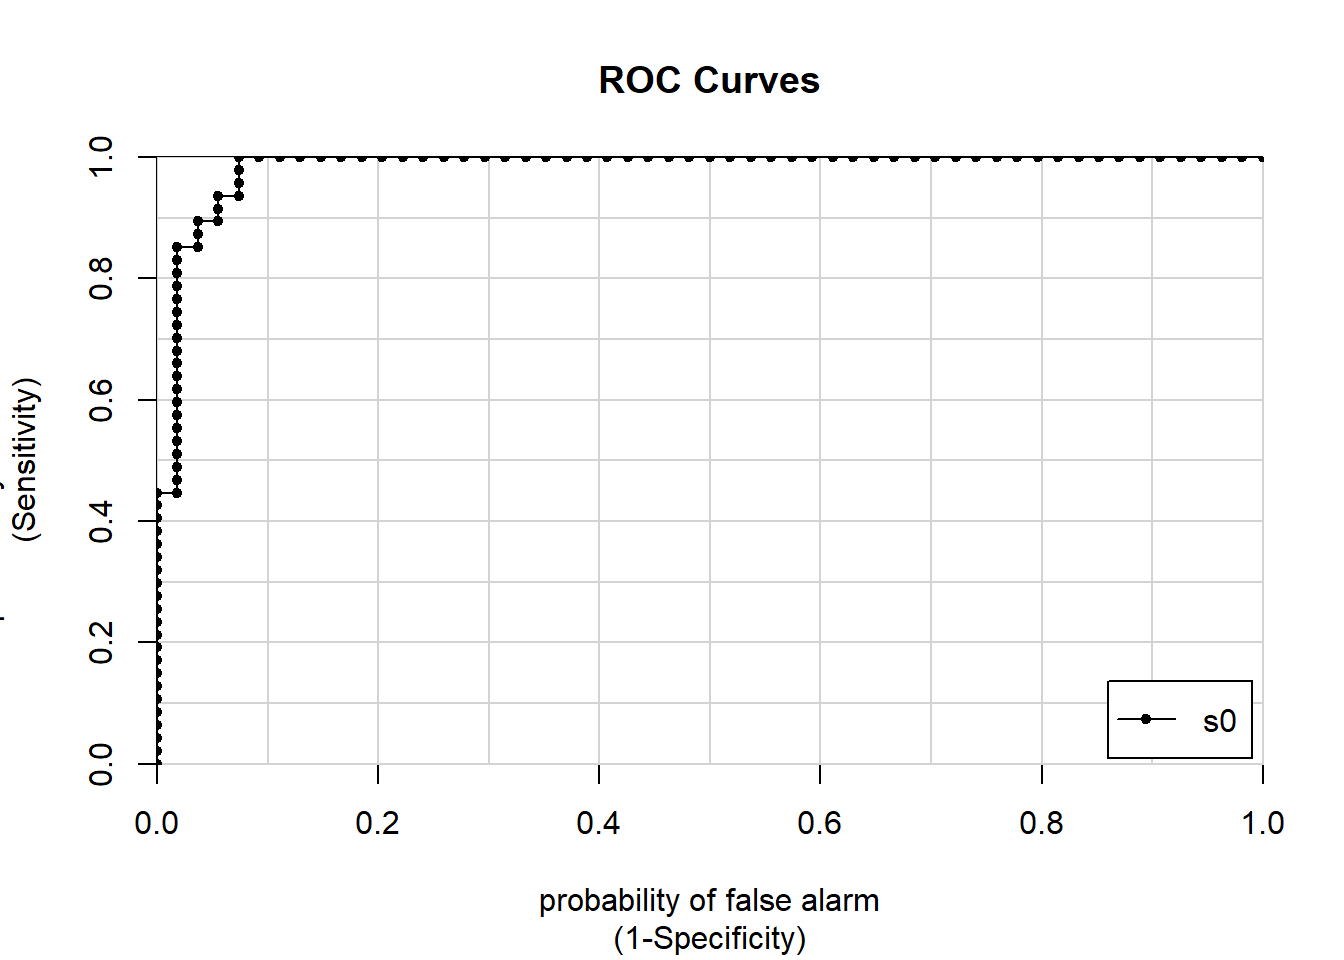
\includegraphics{report_files/figure-latex/unnamed-chunk-9-1.pdf}

\begin{verbatim}
##                           s0
## Latent vs. Primary 0.9838455
\end{verbatim}

This block trains an XGBoost model in order to investigate feature
importance.

\begin{Shaded}
\begin{Highlighting}[]
\NormalTok{labels =}\StringTok{ }\KeywordTok{ifelse}\NormalTok{(mod_df}\OperatorTok{$}\NormalTok{Cohort }\OperatorTok{==}\StringTok{ "Primary"}\NormalTok{, }\DecValTok{1}\NormalTok{, }\DecValTok{0}\NormalTok{)}

\NormalTok{dtrain <-}\StringTok{ }\NormalTok{mod_df }\OperatorTok
\StringTok{  }\KeywordTok{select}\NormalTok{(}\OperatorTok{-}\NormalTok{Cohort) }\OperatorTok\StringTok{ }
\StringTok{  }\KeywordTok{as.matrix}\NormalTok{() }\OperatorTok\StringTok{ }
\StringTok{  }\KeywordTok{xgb.DMatrix}\NormalTok{(}\DataTypeTok{label =}\NormalTok{ labels)}

\NormalTok{xgb_params <-}\StringTok{ }\KeywordTok{list}\NormalTok{(}
  \DataTypeTok{booster =} \StringTok{"gbtree"}\NormalTok{,}
  \DataTypeTok{objective =} \StringTok{"binary:logistic"}
\NormalTok{)}

\NormalTok{model_xgb <-}\StringTok{ }\KeywordTok{xgb.train}\NormalTok{(}
  \DataTypeTok{params =}\NormalTok{ xgb_params,}
  \DataTypeTok{data =}\NormalTok{ dtrain,}
  \DataTypeTok{print_every_n =} \DecValTok{5}\NormalTok{,}
  \DataTypeTok{nrounds =} \DecValTok{60}\NormalTok{,}
  \DataTypeTok{verbose =} \DecValTok{1}
\NormalTok{)}
\end{Highlighting}
\end{Shaded}

This block displays the feature importance metric from XGBoost. This
displays the number of times the tree-based model split on a particular
feature in order to perform classification. The more times a particular
feature is chosen for a split, the more crucial it is to the model.

\begin{Shaded}
\begin{Highlighting}[]
\NormalTok{importance_matrix <-}\StringTok{ }\KeywordTok{xgb.importance}\NormalTok{(}\DataTypeTok{model =}\NormalTok{ model_xgb)}
\KeywordTok{xgb.ggplot.importance}\NormalTok{(importance_matrix)}
\end{Highlighting}
\end{Shaded}

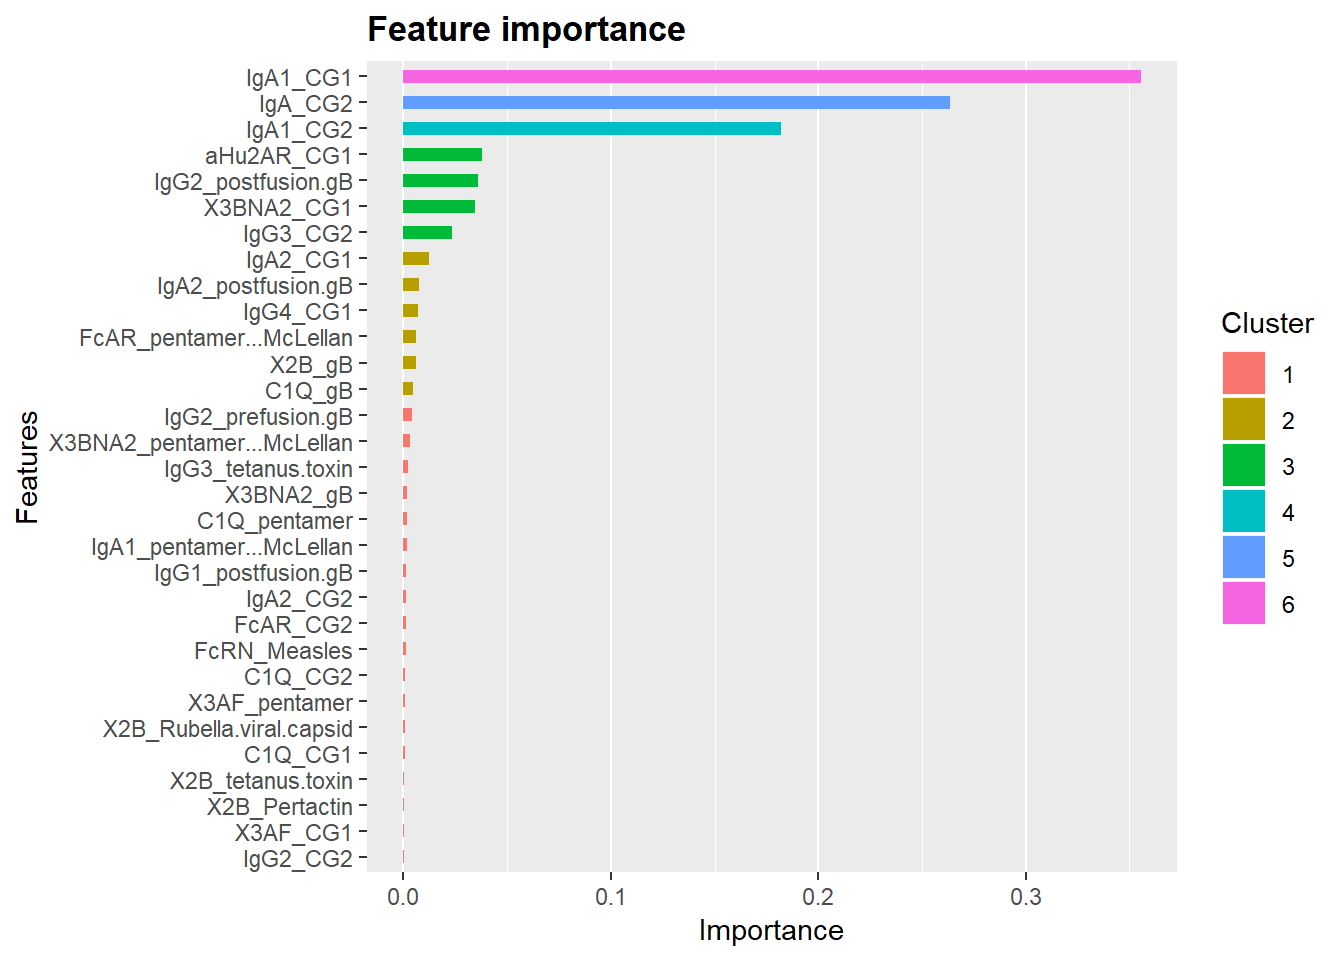
\includegraphics{report_files/figure-latex/unnamed-chunk-11-1.pdf}

The following three plots scatter features chosen by the models as
important against each other. As you can see, there is a lot of
separation in many cases.

\begin{Shaded}
\begin{Highlighting}[]
\KeywordTok{ggplot}\NormalTok{(norm_df, }\KeywordTok{aes}\NormalTok{(}\DataTypeTok{x =}\NormalTok{ IgM.1000f_gB, }\DataTypeTok{y =}\NormalTok{ IgM.1000f_postfusion.gB, }\DataTypeTok{color =}\NormalTok{ Cohort)) }\OperatorTok{+}
\StringTok{  }\KeywordTok{geom_point}\NormalTok{() }\OperatorTok{+}
\StringTok{  }\KeywordTok{labs}\NormalTok{(}\DataTypeTok{title =} \StringTok{"IgM.1000f_postfusion.gB vs. IgM.1000f_gB"}\NormalTok{)}
\end{Highlighting}
\end{Shaded}

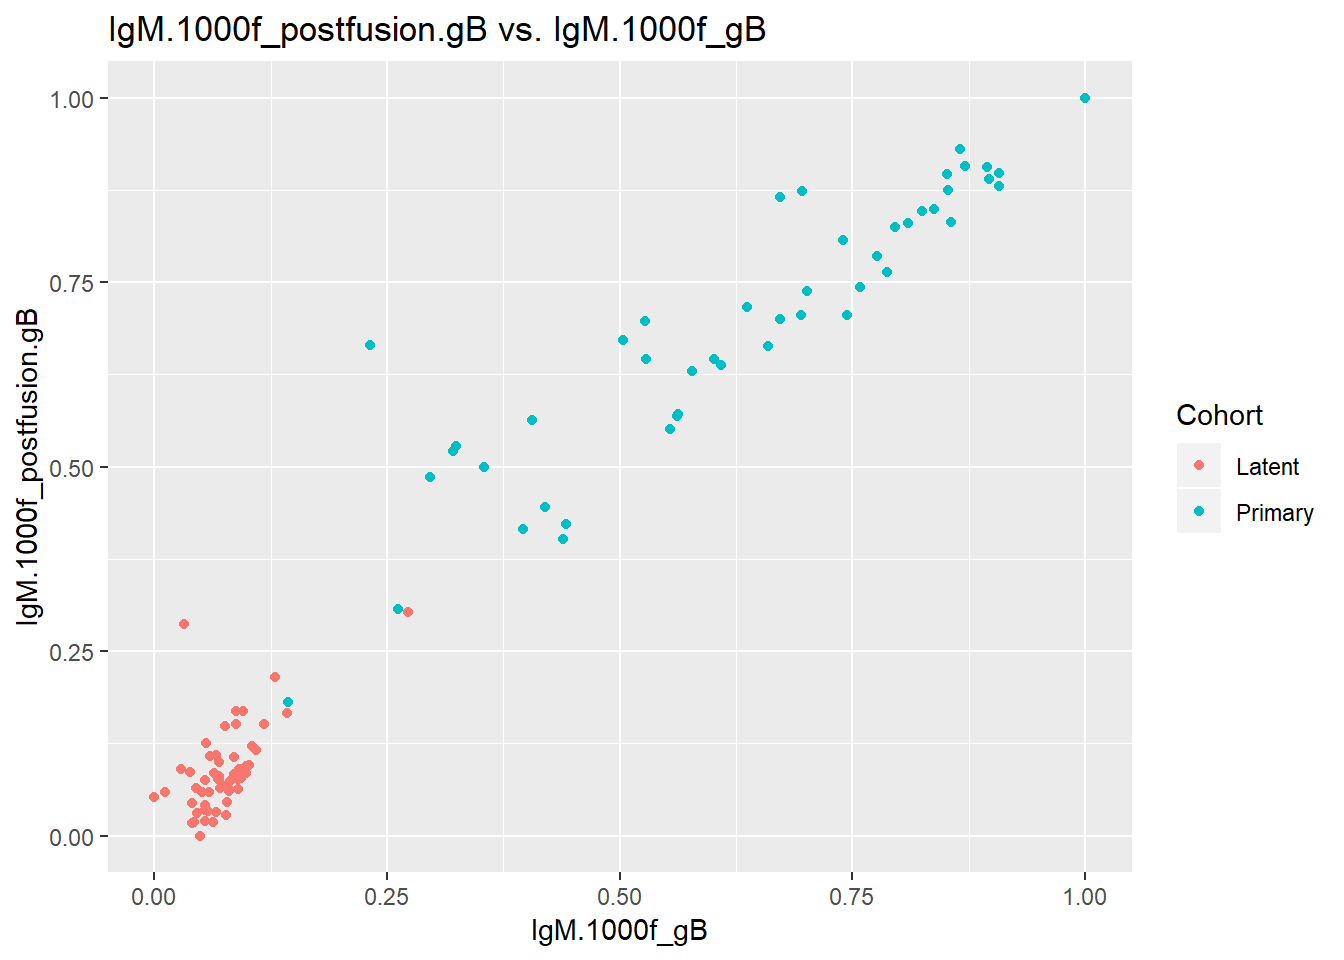
\includegraphics{report_files/figure-latex/unnamed-chunk-12-1.pdf}

\begin{Shaded}
\begin{Highlighting}[]
\KeywordTok{ggplot}\NormalTok{(norm_df, }\KeywordTok{aes}\NormalTok{(}\DataTypeTok{x =}\NormalTok{ IgA2_CG2, }\DataTypeTok{y =}\NormalTok{ IgA1_CG1, }\DataTypeTok{color =}\NormalTok{ Cohort)) }\OperatorTok{+}
\StringTok{  }\KeywordTok{geom_point}\NormalTok{() }\OperatorTok{+}
\StringTok{  }\KeywordTok{labs}\NormalTok{(}\DataTypeTok{title =} \StringTok{"IgA1_CG1 vs. IgA2_CG2"}\NormalTok{)}
\end{Highlighting}
\end{Shaded}

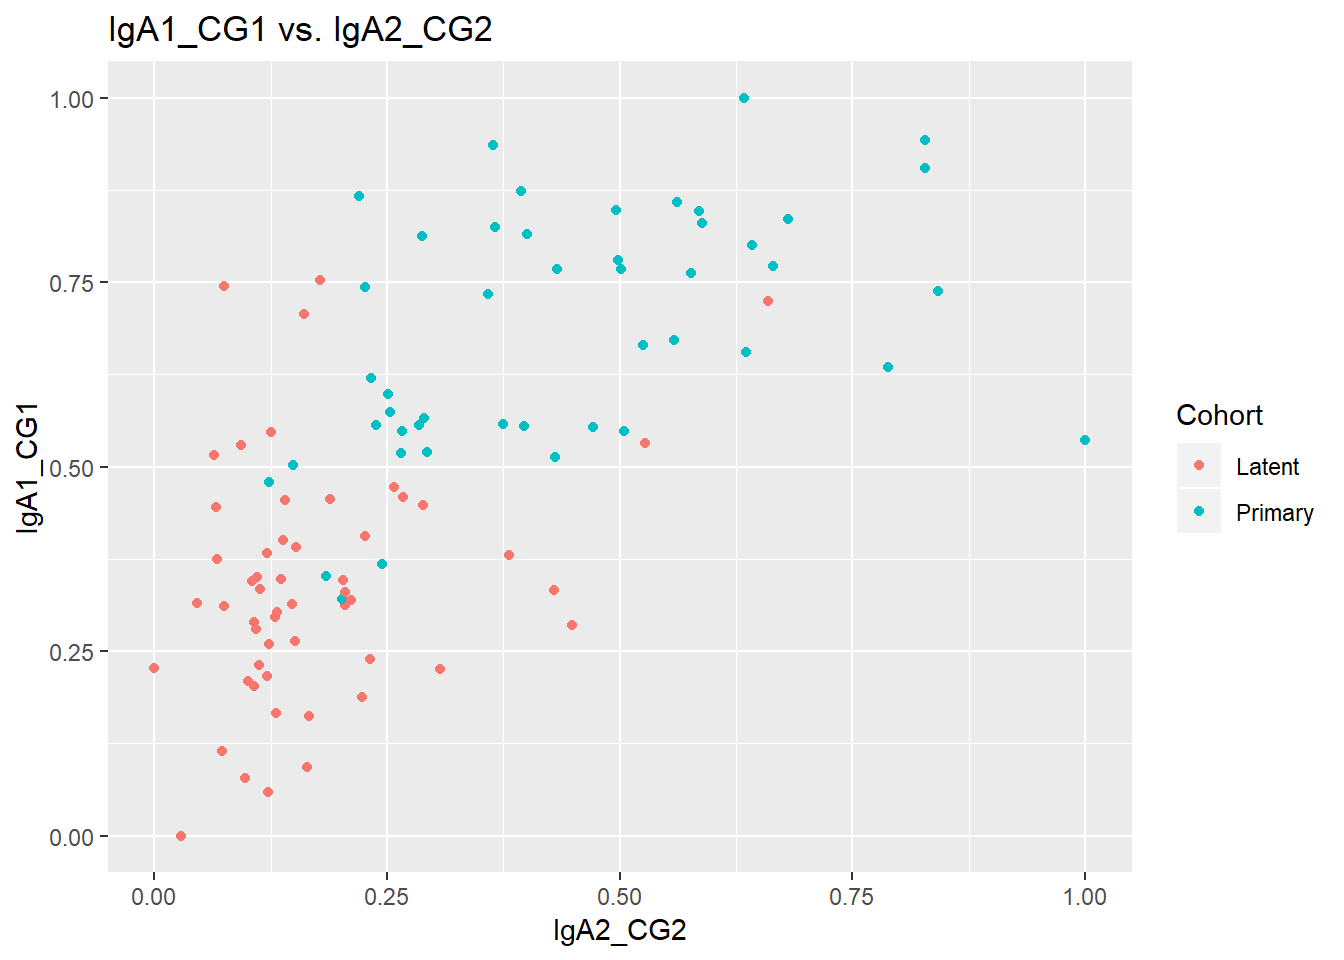
\includegraphics{report_files/figure-latex/unnamed-chunk-13-1.pdf}

\begin{Shaded}
\begin{Highlighting}[]
\KeywordTok{ggplot}\NormalTok{(norm_df, }\KeywordTok{aes}\NormalTok{(}\DataTypeTok{x =}\NormalTok{ IgG3_pentamer, }\DataTypeTok{y =}\NormalTok{ IgA1_CG1, }\DataTypeTok{color =}\NormalTok{ Cohort)) }\OperatorTok{+}
\StringTok{  }\KeywordTok{geom_point}\NormalTok{() }\OperatorTok{+}
\StringTok{  }\KeywordTok{labs}\NormalTok{(}\DataTypeTok{title =} \StringTok{"IgA1_CG1 vs. IgG3_pentamer"}\NormalTok{)}
\end{Highlighting}
\end{Shaded}

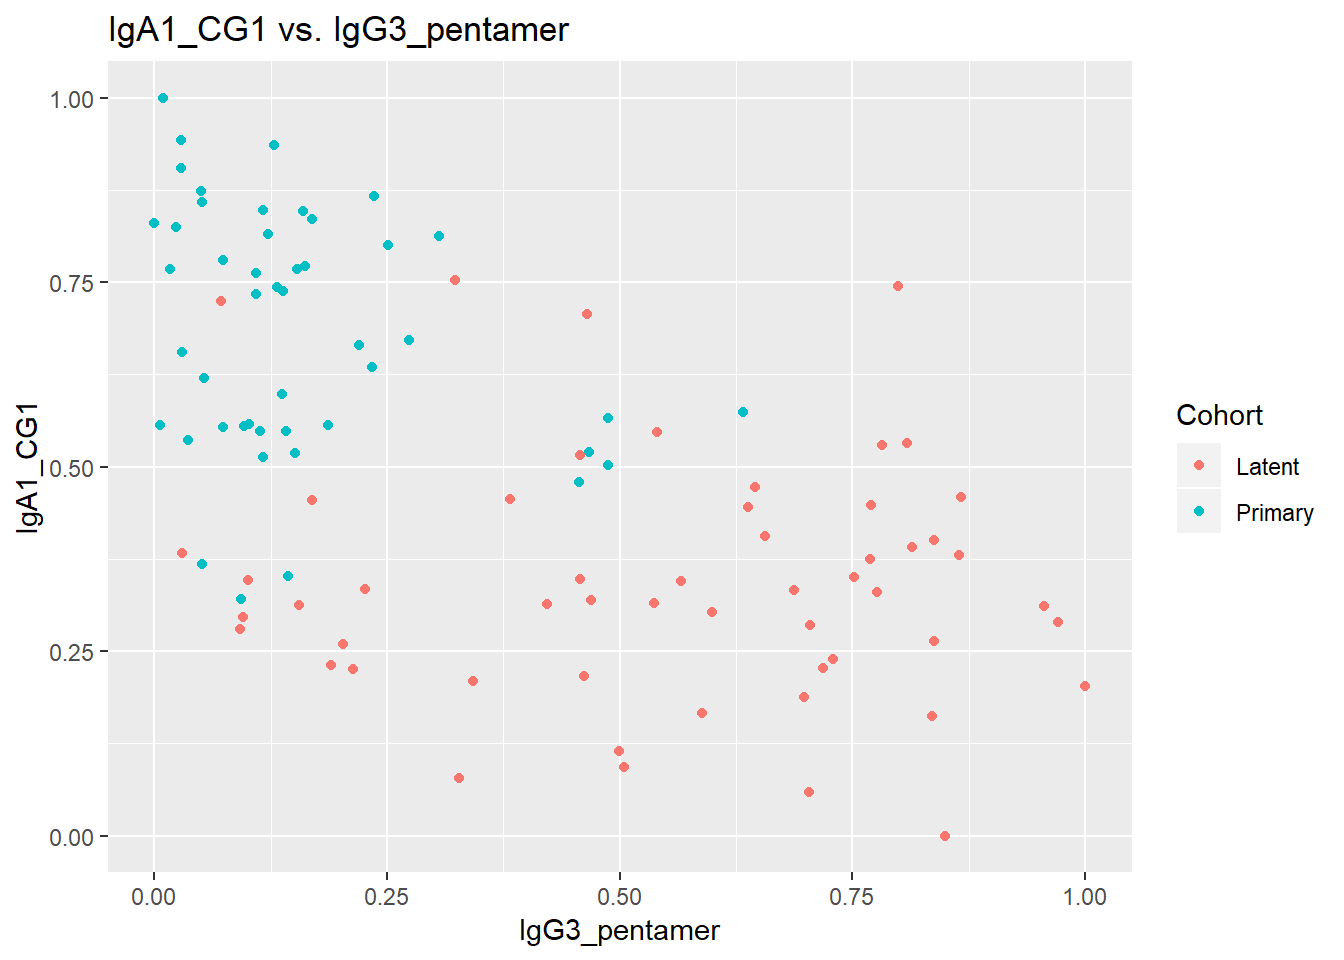
\includegraphics{report_files/figure-latex/unnamed-chunk-14-1.pdf}


\end{document}
